\documentclass[conference]{IEEEtran}
\IEEEoverridecommandlockouts
% The preceding line is only needed to identify funding in the first footnote. If that is unneeded, please comment it out.
\usepackage{cite}
\usepackage{amsmath,amssymb,amsfonts}
\usepackage{algorithmic}
\usepackage{graphicx}
\usepackage{textcomp}
\usepackage{xcolor}
\usepackage{booktabs}
\usepackage[table]{xcolor}
\usepackage{siunitx}
\usepackage{threeparttable}
\usepackage{svg}

\usepackage{multirow}   
\usepackage{url}
\def\BibTeX{{\rm B\kern-.05em{\sc i\kern-.025em b}\kern-.08em
    T\kern-.1667em\lower.7ex\hbox{E}\kern-.125emX}}
\DeclareMathOperator*{\argmax}{argmax} % thin space, limits underneath in displays


\begin{document}



\title{Scalable Traffic Prediction via Data Reduction with Coreset Selection}


\author{\IEEEauthorblockN{1\textsuperscript{st} Taeyoung Yu}
\IEEEauthorblockA{\textit{The University of Queensland} \\
Brisbane, Australia \\
taeyoung.yu@uq.edu.au}
\and
\IEEEauthorblockN{2\textsuperscript{nd} Jiwon Kim}
\IEEEauthorblockA{\textit{The University of Queensland} \\
Brisbane, Australia \\
jiwon.kim@uq.edu.au}
\and
\IEEEauthorblockN{3\textsuperscript{rd} Soban Nasir Lone}
\IEEEauthorblockA{\textit{Technical University of Munich} \\
Munich, Germany \\
soban.lone@tum.de}
\and
\IEEEauthorblockN{4\textsuperscript{th} Mohamed Abouelela}
\IEEEauthorblockA{\textit{Technical University of Munich} \\
Munich, Germany \\
mohamed.abouelela@tum.de}
\and
\IEEEauthorblockN{5\textsuperscript{th} Constantinos Antoniou}
\IEEEauthorblockA{\textit{Technical University of Munich} \\
Munich, Germany \\
c.antoniou@tum.de}}
\maketitle


\begin{abstract}
Deep learning models for large-scale traffic forecasting require significant computation for training massive datasets. Coreset selection, which selects small representative data subsets, can reduce computational burden while maintaining prediction accuracy. We comprehensively evaluated eight model-free coreset selection methods for short-term traffic flow prediction, using a Spatio-Temporal Graph Convolutional Network (STGCN) model on the PEMS04 and PEMS07 datasets. Our experiments show that predictive performance comparable to the full dataset model can be maintained with only 30-50\% of the data, without a significant performance drop. Furthermore, using 50-90\% of the data sometimes leads to slightly better performance than training on the entire dataset. The clustering-based approach achieved the highest overall accuracy, suggesting that clustering can effectively select representative samples while filtering out noisy samples. Our analysis indicates that feature space coverage is connected to coreset selection performance and that temporal diversity can be utilised to enhance this coverage. Coresets with strong temporal bias performed poorly, failing to achieve broad feature-space coverage.
\end{abstract}

\begin{IEEEkeywords}
traffic prediction, coreset selection, data-efficient learning, deep learning, multivariate time series prediction
\end{IEEEkeywords}

\section{Introduction}
The advancement of Intelligent Transportation Systems (ITS) has increased the importance and applicability of traffic prediction. Traffic prediction plays a pivotal role in enhancing road traffic efficiency and driver experience, supporting applications such as travel time estimation, congestion management, route guidance, and signal control for effective traffic flow management \cite{vlahogianni_short-term_2014}.
% Also, developments in Internet of Things (IoT) technologies have grown the volume and variety of data collected within the transportation domain. 
The availability of extensive traffic data, particularly from network-wide loop detectors, has enhanced the development and validation of traffic prediction models.
For example, the Performance Measurement System (PEMS) provides link-level traffic data such as flow, speed, and density (occupancy)  at 5-minute intervals from thousands of loop detectors deployed across road networks \cite{chen_freeway_2001}, covering freeways across major metropolitan areas of California, USA, as shown in Figure~\ref{fig:sensor_maps}.

\begin{figure}[htbp]
  \centering
  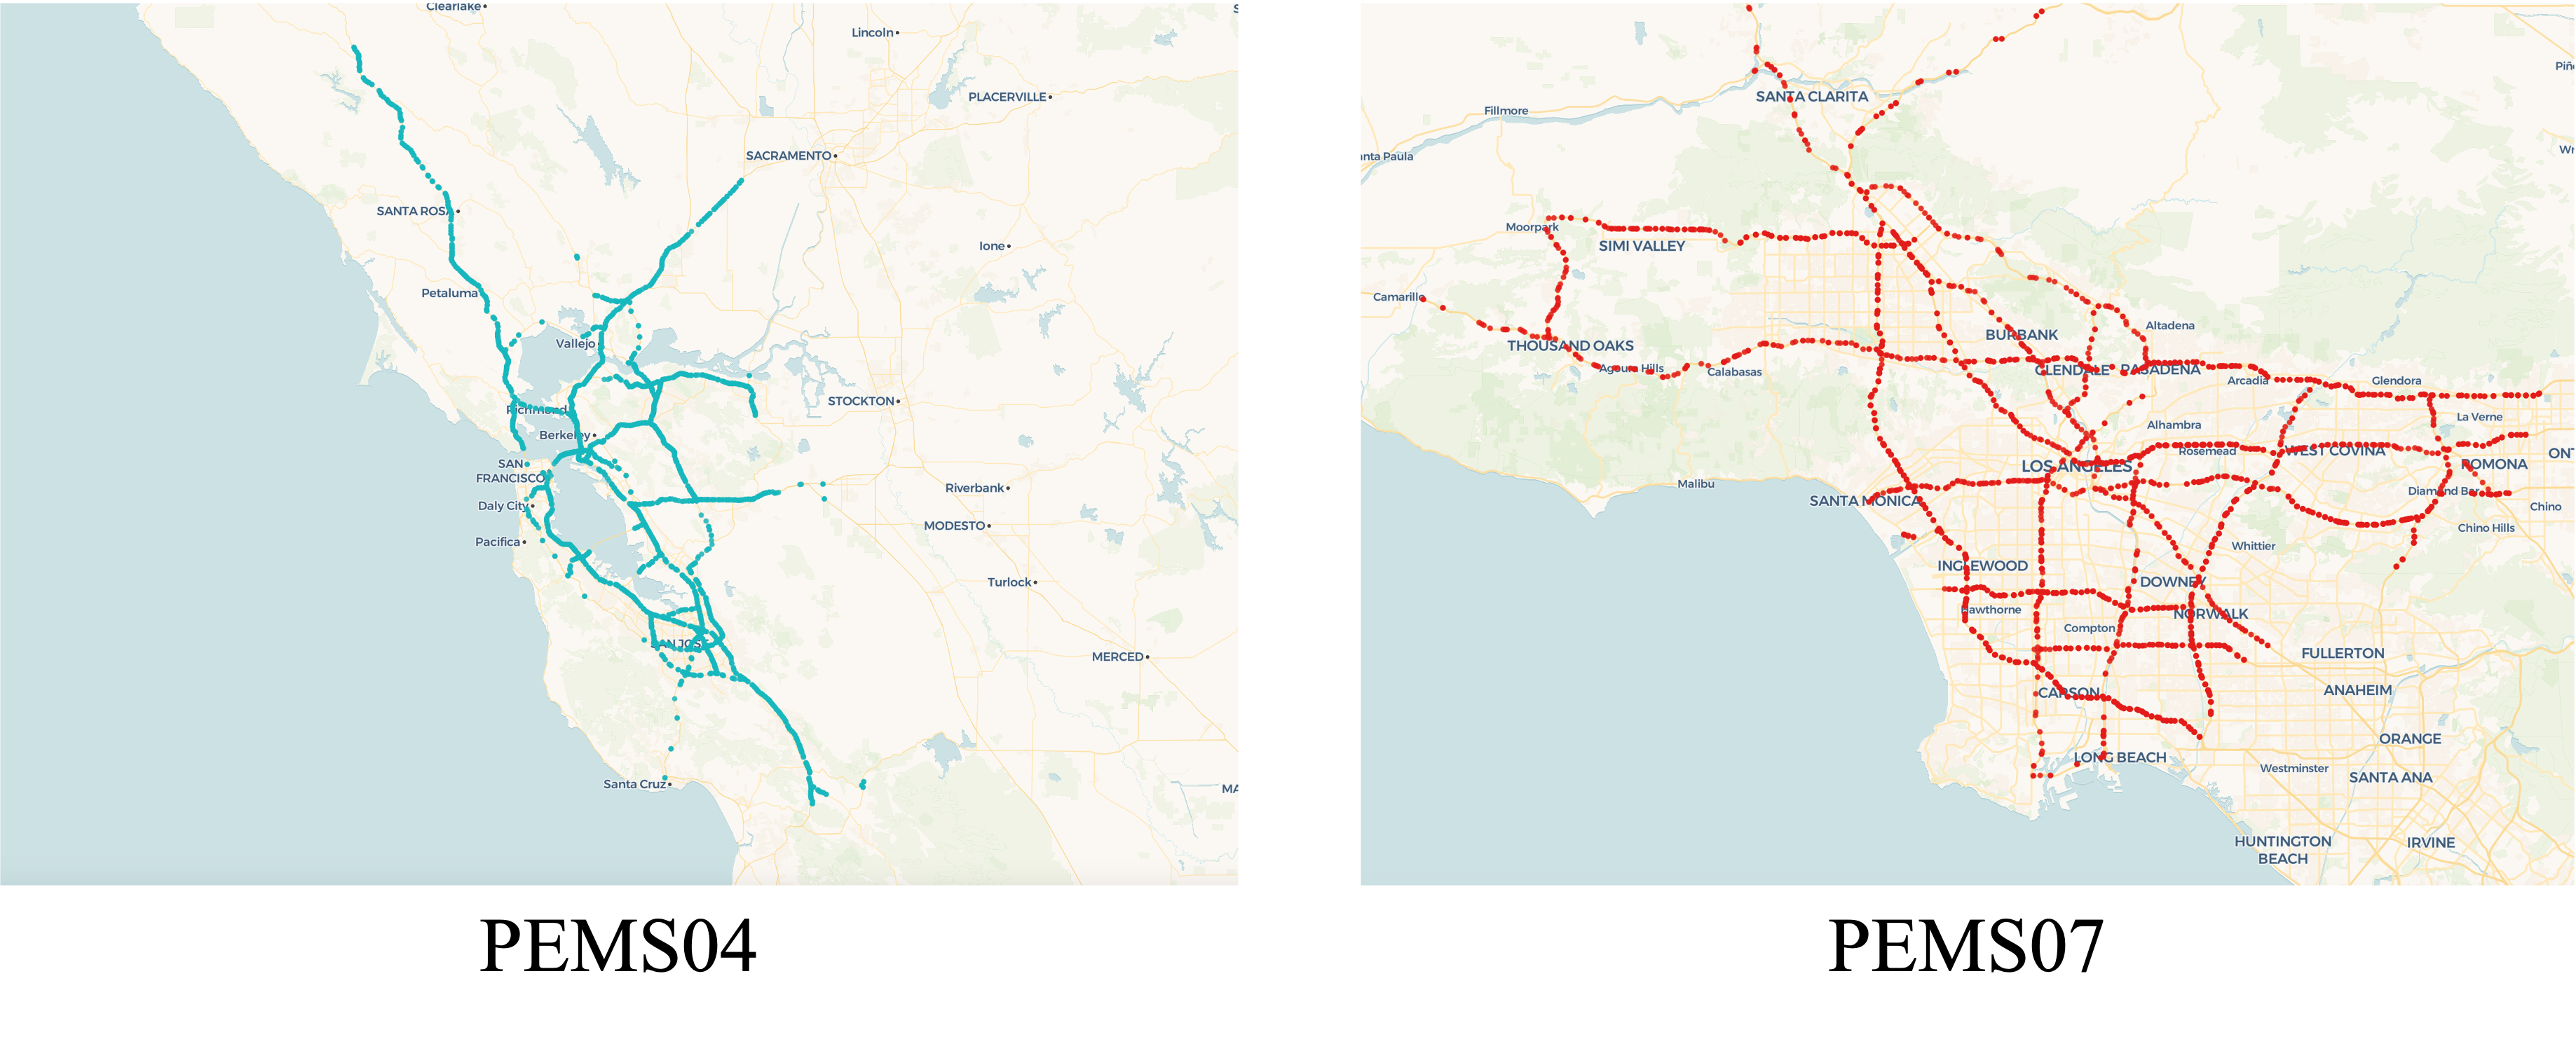
\includegraphics[width=0.9\linewidth]{figures/sensor_map.png} 
  \caption{Geographical distribution of traffic sensors in the PEMS04 (left, Bay Area) and PEMS07 (right, Los Angeles) datasets evaluated in this study.}
  \label{fig:sensor_maps}
\end{figure}

Recent innovations in machine learning have investigated application of Graph Neural Networks (GNNs) for traffic prediction \cite{yin_deep_2021}. These models capture the complex spatio-temporal dependencies in traffic data and have demonstrated superior performance compared to traditional time-series forecasting methods such as Autoregressive Integrated Moving Average (ARIMA) and other machine learning models for sequential prediction such as Long Short-Term Memory (LSTM)~\cite{wu_graph_2019, cui_traffic_2019}. However, GNN models require substantial training data and extensive computation, causing challenges related to training time and resources.
Recent benchmark study shows several state-of-the-art GNNs suffer from long training time due to their increased model complexity\cite{liu_largest_2023}.
% either require more than 100 GPU-hours or cannot be trained at all within practical resource limits \cite{liu_largest_2023}.

In computer vision research area, various techniques have been proposed to lower the computational burden associated with training complex models on large datasets. \textit{Coreset} selection, the task of identifying a small, representative subset of data samples from original dataset, has demonstrated significant advances in image classification tasks. Applied to benchmarks like CIFAR-10, CIFAR-100, and ImageNet-1k, it has demonstrated the potential to significantly reduce training resources with minimal impact on model performance. Recent studies \cite{xia_moderate_2022, maharana_d2_2023, tan_data_2025} indicate that models trained on coresets using only 50\% of the original data can achieve predictive performance with only a small degradation (e.g., less than a 5\% drop). Minimising the dataset size with small performance loss offers decreased training time and computational cost. This accelerates model development and deployment cycle, by enabling faster experimentation and optimisation.

In contrast, applying coreset selection to multivariate time-series forecasting such as traffic prediction has received limited attention. Multivariate time-series data commonly contain strong periodicities (e.g., daily, weekly cycles), creating data redundancy. At the same time, these datasets frequently include unique but potentially important events or anomalies. Therefore, the selection of coreset in this domain must balance reducing data redundancy and keeping essential pattern information.
Thus, systematically investigating coreset selection for large-scale multivariate time-series forecasting can improve computational efficiency and forecasting accuracy, opening diverse application opportunities.

In this paper, we present a comprehensive investigation into the application of coreset selection methods for traffic prediction. We evaluated eight coreset selection methods. We apply these methods to the traffic prediction task based on a GNN model using two benchmark datasets. Our findings shed light on both the potential benefits and limitations of employing coreset selection in traffic forecasting. 

\begin{figure*}[t] 
  \centering
  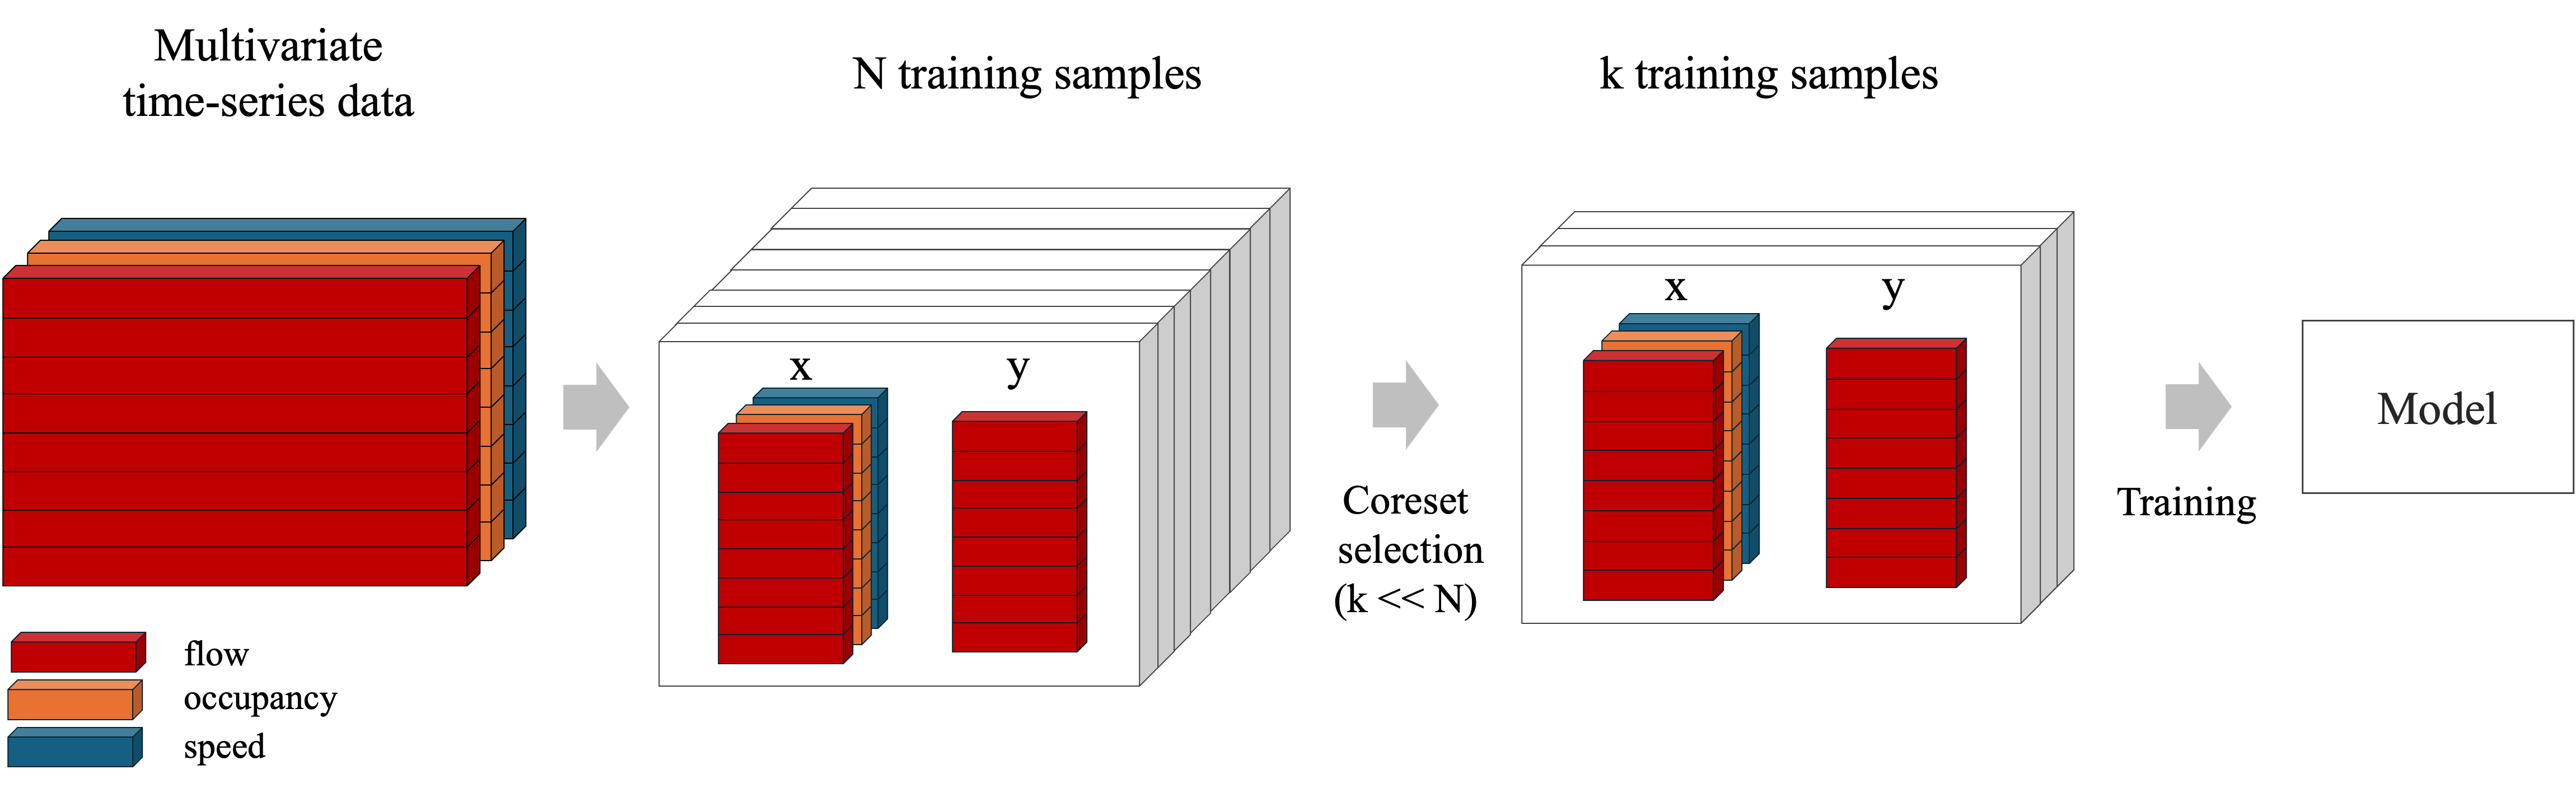
\includegraphics[width=\linewidth]{figures/overall.png} 
  \caption{Overall pipeline of applying coreset selection for traffic forecasting model training.}
  \label{fig:overall_workflow}
\end{figure*}
% ----------------------------------

The main contributions of this paper can be summarised as follows:
\begin{itemize}
    \item To the best of our knowledge, we present the first systematic benchmark evaluating eight model-free coreset selection methods for large-scale GNN-based traffic forecasting. 
    \item We demonstrate that model performance using a coreset depends on achieving good feature‐space coverage. Furthermore, we show that for spatio-temporal traffic data, preserving temporal diversity is an effective strategy to help attain this crucial feature coverage.

    \item We empirically validate that using only 30-50\% coresets maintains prediction accuracy near the accuracy of full-data baseline. We also observe that certain coresets (often 50-90\% ratio) slightly outperformed models trained on the entire dataset.
\end{itemize}
\section{Related Works}
This section reviews previous work in two key areas relevant to our study: deep learning models for traffic prediction and coreset selection selection.

\subsection{Deep Learning Models for Traffic Prediction}\label{sec:traffic_forecasting}
Traffic forecasting is a multivariate spatio-temporal time–series problem to predict future traffic states (e.g., speed, flow, occupancy) in multiple locations. Since traffic states are influenced by both adjacent locations and past states, it is important to capture (i) spatial correlations among locations and (ii) temporal patterns across different horizons.

GNNs have become an emerging model for traffic forecasting since they can model the road network explicitly as a graph whose nodes represent sensors on road segments and edges represent connectivity between road segments. Especially, spatio-temporal GNNs have made significant progress in recent years by capturing hidden patterns of spatial-temporal graphs \cite{wu_graph_2019}, \cite{yu_spatio-temporal_2018}, \cite{cui_traffic_2019}, \cite{li_dynamic_2023}, \cite{bai_adaptive_2020}.


However, compared to simpler models, GNNs generally rely on a higher computational burden during the training phase. Recent benchmark results show that training the state-of-the-art GNN model on one year’s data from 2,352 sensors requires 148 GPU-hours on a single GPU \cite{liu_largest_2023}. To address these computational bottlenecks, efficient learning paradigms have been proposed, including model compression and architectural optimisation \cite{zheng_lightcast_2024, zhang_efficient_2025}. 

\subsection{Coreset Selection}
Coreset selection aims to select a small but representative subset of a given dataset, while minimising the performance drop observed when training a model using the subset compared to training using the entire dataset. This technique directly reduces the computational burden associated with training complex models on massive datasets. Many previous research studied coreset selection in the image classification domain. They can be categorised into two main categories: \textit{Model-free} methods and \textit{Model-dependent} methods.

\subsubsection{Model-free coreset selection}
These methods select coresets purely based on data characteristics (e.g., distance metrics, similarity), without requiring model training or gradient information.
\begin{itemize}
    \item \textbf{Geometric methods:} Select a coreset using geometric measures like distances between data samples. For example, \textit{k-center greedy} \cite{sener_active_2018} iteratively selects data sample farthest from each step's coreset and \textit{herding} \cite{welling_herding_2009} constructs a coreset by iteratively adding data samples to match the average moment of the selected samples with the entire dataset's average moment.
    \item \textbf{Submodular methods:} Select a coreset using a submodular function, which measures overall information of given subset. For example, \textit{facility-location} \cite{kothawade_prism_2022}, selects data samples that best "cover" the dataset based on a similarity measure.
\end{itemize}
These methods are generally computationally efficient, which makes them particularly suitable for large-scale datasets.

\subsubsection{Model-dependent coreset selection}
These methods utilise information from a trained model (e.g., gradients, losses, representations) to select coresets. They evaluate each data point under the model to choose the most informative subset and, thus, generally bring higher computational costs during the selection phase :

\begin{itemize}
    \item \textbf{Gradient-based methods:} Select a coreset whose aggregated gradients approximate the full data gradient. For instance, \textit{CRAIG} \cite{mirzasoleiman_coresets_2020} selects a coreset by greedily maximizing a submodular facility location function defined over distances between gradients. \textit{GradMatch} \cite{killamsetty_grad-match_2021} selects a subset by using orthogonal matching to align the subset's weighted gradient sum with a target gradient.
    %(full training or validation).

    \item \textbf{Score-based methods:} Select a coreset based on an importance score of each data point, such as prediction error, loss magnitude, gradient norm, or training dynamics. For instance, \textit{EL2N} \cite{paul_deep_2021} measures importance scores using squared L2 norm of the prediction error vector, and \textit{GraNd} \cite{paul_deep_2021} uses gradient norm of the loss of each training samples. \textit{Forgetting} \cite{toneva_empirical_2018} counts how often each sample switches from correct to incorrect during training. \textit{CCS} \cite{zheng_coverage-centric_2022} conducts stratified sampling based on importance scores to improve data coverage.


    \item \textbf{Hybrid methods: } Combine model-derived information, such as learned representations or losses, with geometric principles like diversity or coverage. For instance, \textit{Moderate} \cite{xia_moderate_2022} measures the distance of each sample to its class center using extracted representation and selects samples near the median distance. \textit{D2 Pruning} \cite{maharana_d2_2023} applies a message passing approach based on embedding space, for balancing difficulty and diversity. \textit{Infomax} \cite{tan_data_2025} selects a coreset by formulating the problem as maximizing the sum of individual sample importance scores while penalizing pairwise similarities within the subset.
\end{itemize}

The primary motivation for using coresets in large-scale traffic forecasting is to reduce computational overhead. Since \textit{model-dependent} methods require additional resources for model training during the selection process, we focus on evaluating \textit{model-free} coreset selection methods in this paper.
\section{Preliminaries}

\subsection{Traffic Flow Prediction}

The objective of traffic flow prediction is to predict the target flow in future steps based on historical observations over a sensor network. Given a window length $T_{in}$ for the input data, traffic prediction aims to predict future traffic flow values for the next $T_{out}$ timestamps. 

Let \(\mathbf X\in\mathbb R^{N\times T\times F}\) denote the multivariate time series data collected from \(N\) sensors over \(T\) time steps with \(F\) features (e.g., flow, speed, occupancy).

\begin{equation}\label{eq:forecast_centered}
\begin{gathered}
  \hat{\mathbf{Y}}_{t : t+T_{\text{out}}-1}
      = f_{\theta}\!\left(\mathbf{X}_{t-T_{\text{in}} : t-1}\right)
      \\[6pt]
  \text{for } T_{\text{in}} + 1 \le t \le T - T_{\text{out}} + 1 .
\end{gathered}
\end{equation}
%
Here, \(\hat{\mathbf{Y}} \in \mathbb{R}^{N \times T_{\text{out}} \times 1}\) is the predicted traffic flow sequence. The learning pipeline updates the parameters \(\boldsymbol{\theta}\) of the function \(f_{\theta}\) by minimising a loss function \(\mathcal{L}(\hat{\mathbf{Y}}, \mathbf{Y})\), with ground-truth target data \(\mathbf{Y} \in \mathbb{R}^{N \times T_{\text{out}} \times 1}\). 


\subsection{Coreset Selection}

Given the entire training dataset $D_{train} = \{(\mathbf{X}_i, \mathbf{Y}_i)\}_{i=1}^{|D_{train}|}$, consisting of pairs of historical input sequences $\mathbf{X}_i$ and their corresponding future traffic flow sequences $\mathbf{Y}_i$, \textit{coreset selection} aims to identify a smaller and representative subset $S \subseteq D_{train}$ of size $|S| < |D_{train}|$. Given a desired coreset size $k$, the optimal coreset $S^*$ is defined as the training data subset of size $k$, i.e., $|S^*|=k$ that maximises prediction performance on an independent test dataset $D_{test}$:
\begin{equation}
S^* = \argmax_{S \subseteq D_{train},\, |S| = k} \mathrm{Perf}(f_{\theta_S}, D_{test})
\end{equation}
%
where $f_{\theta_S}$ denotes a prediction model trained on the coreset $S$. The performance metric $\mathrm{Perf}(\cdot)$ typically measures predictive accuracy. Figure~\ref{fig:overall_workflow} illustrates the overall pipeline for coreset selection in this study.

\begin{figure*}[t] 
  \centering
  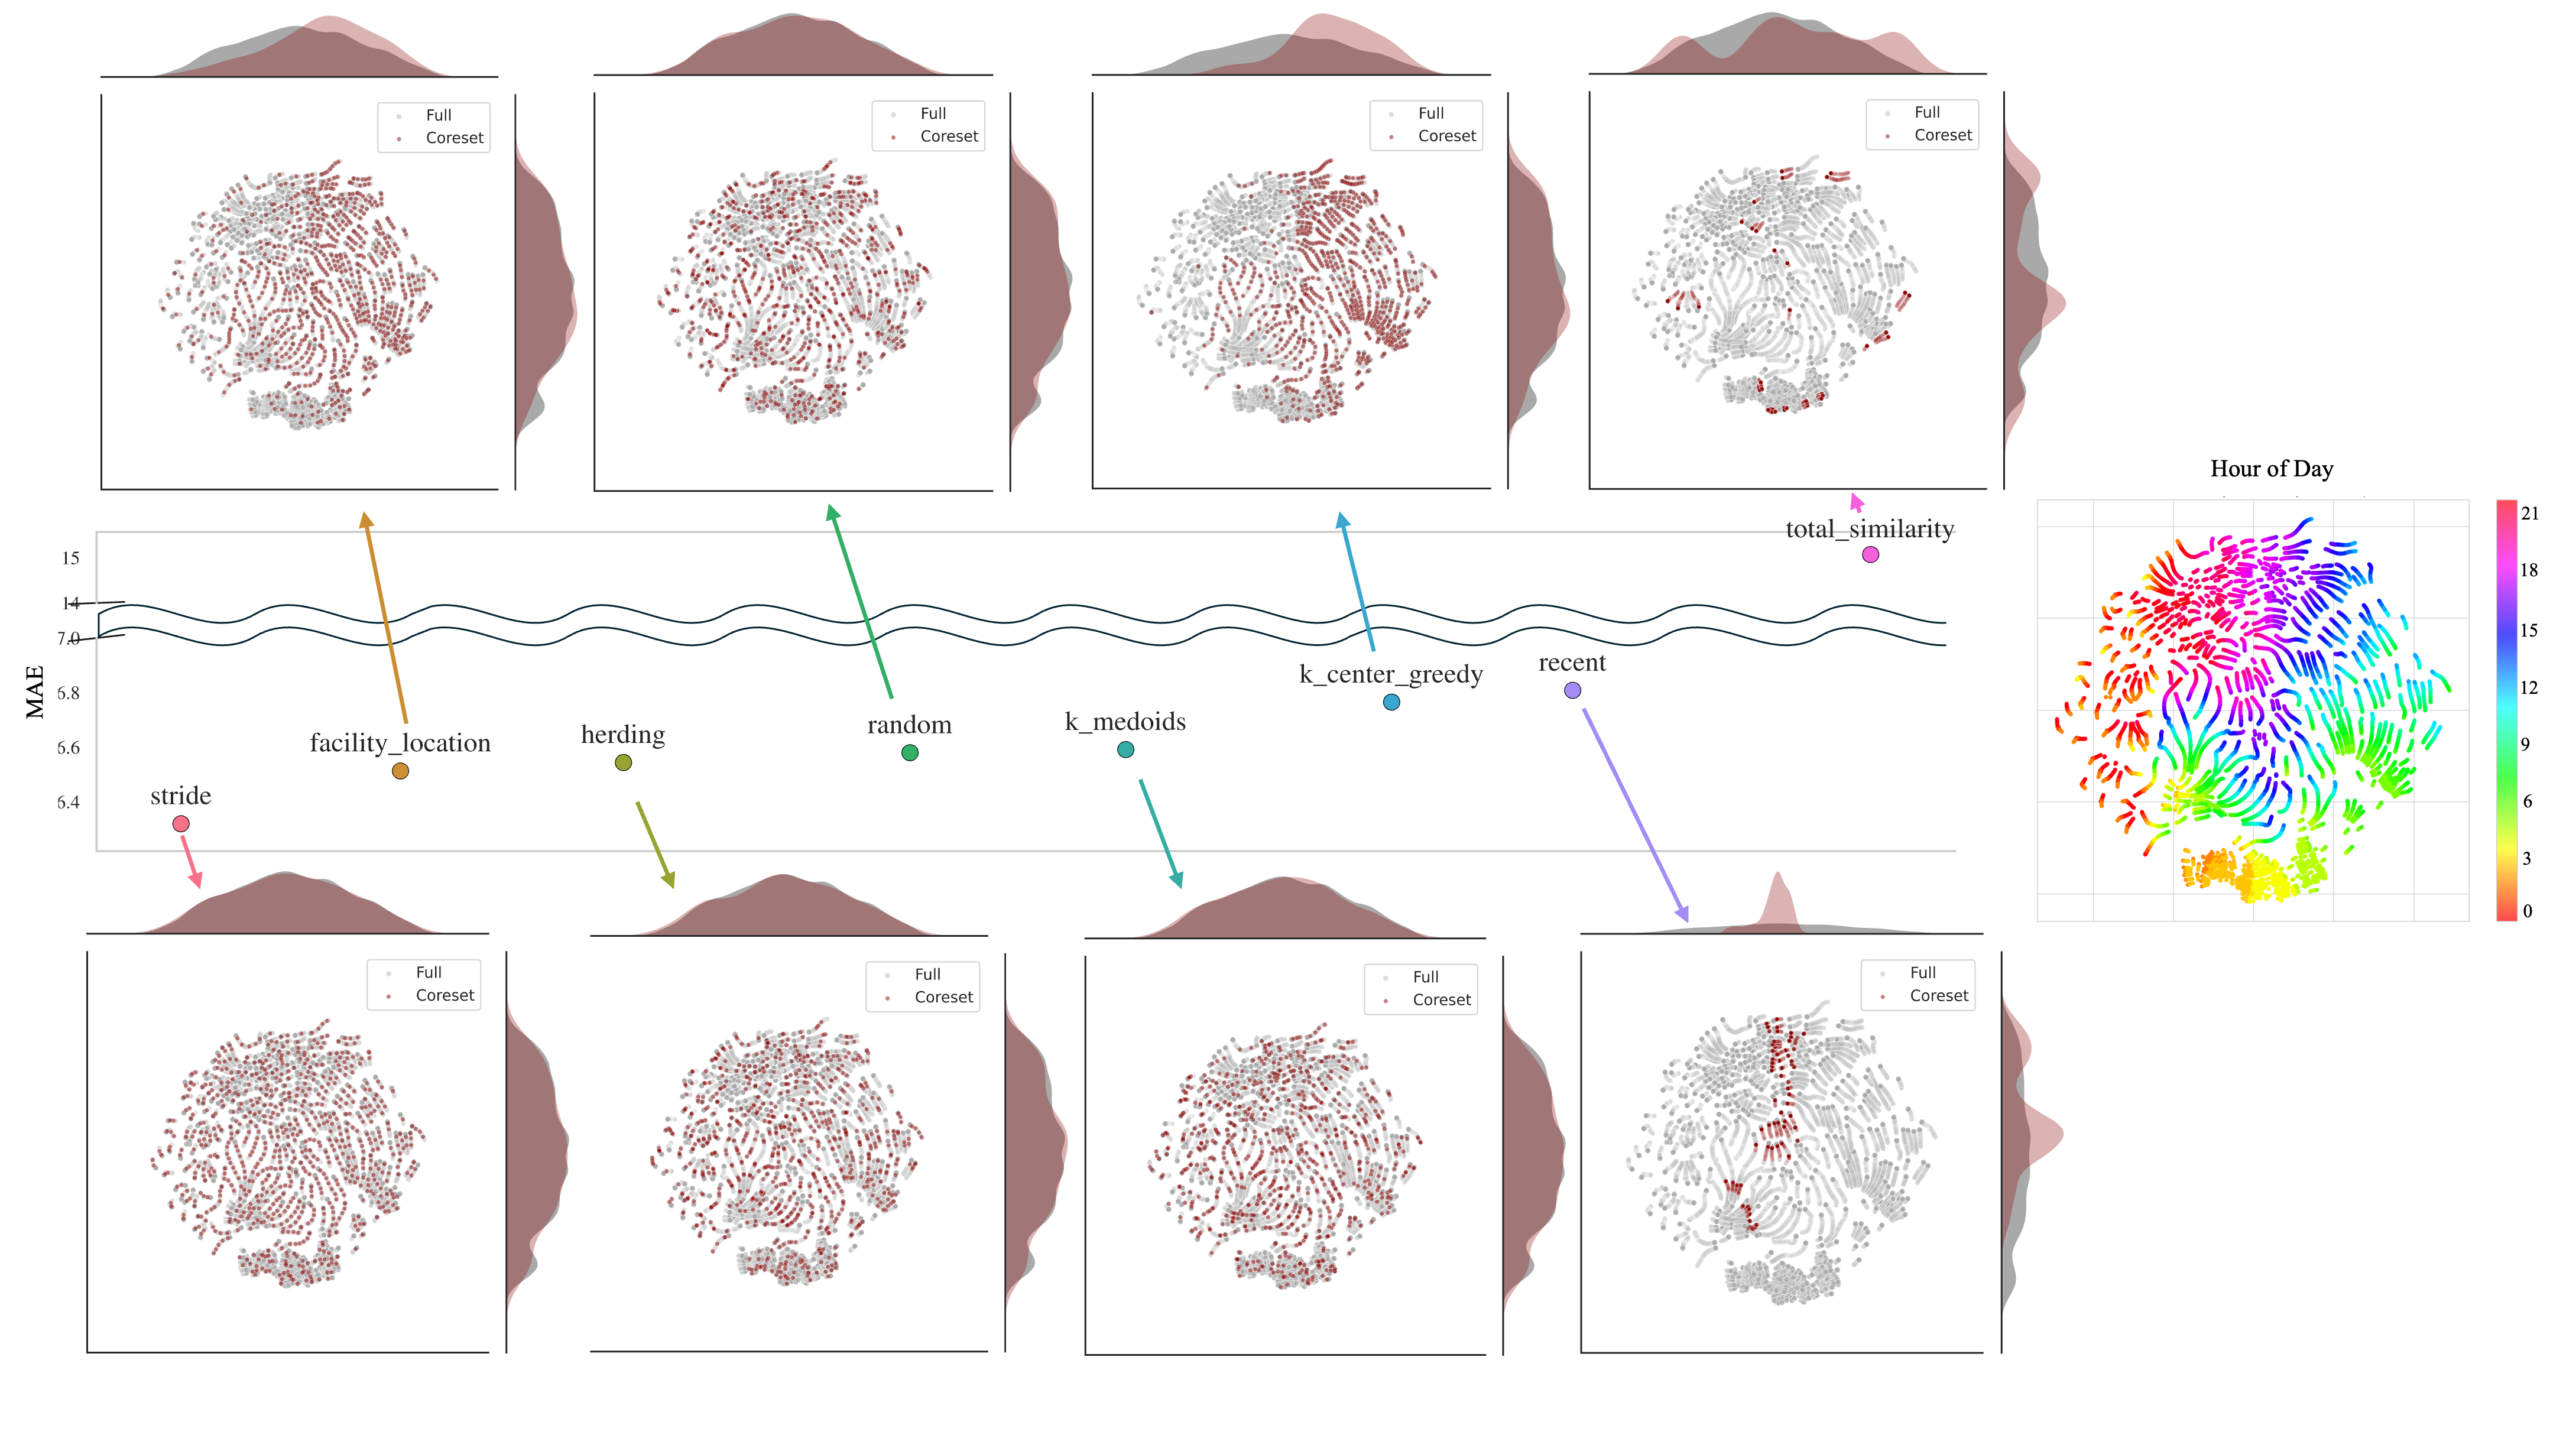
\includegraphics[width=\textwidth]{figures/tsne.png} 
  \caption{t-SNE visualization (center plots) and Kernel Density Estimates (marginal plots) of the full dataset (grey/darker shade) and the selected coresets (red/lighter shade) for each selection method.} 
  \label{fig:tsne}
\end{figure*}

\begin{figure*}[t] 
  \centering
  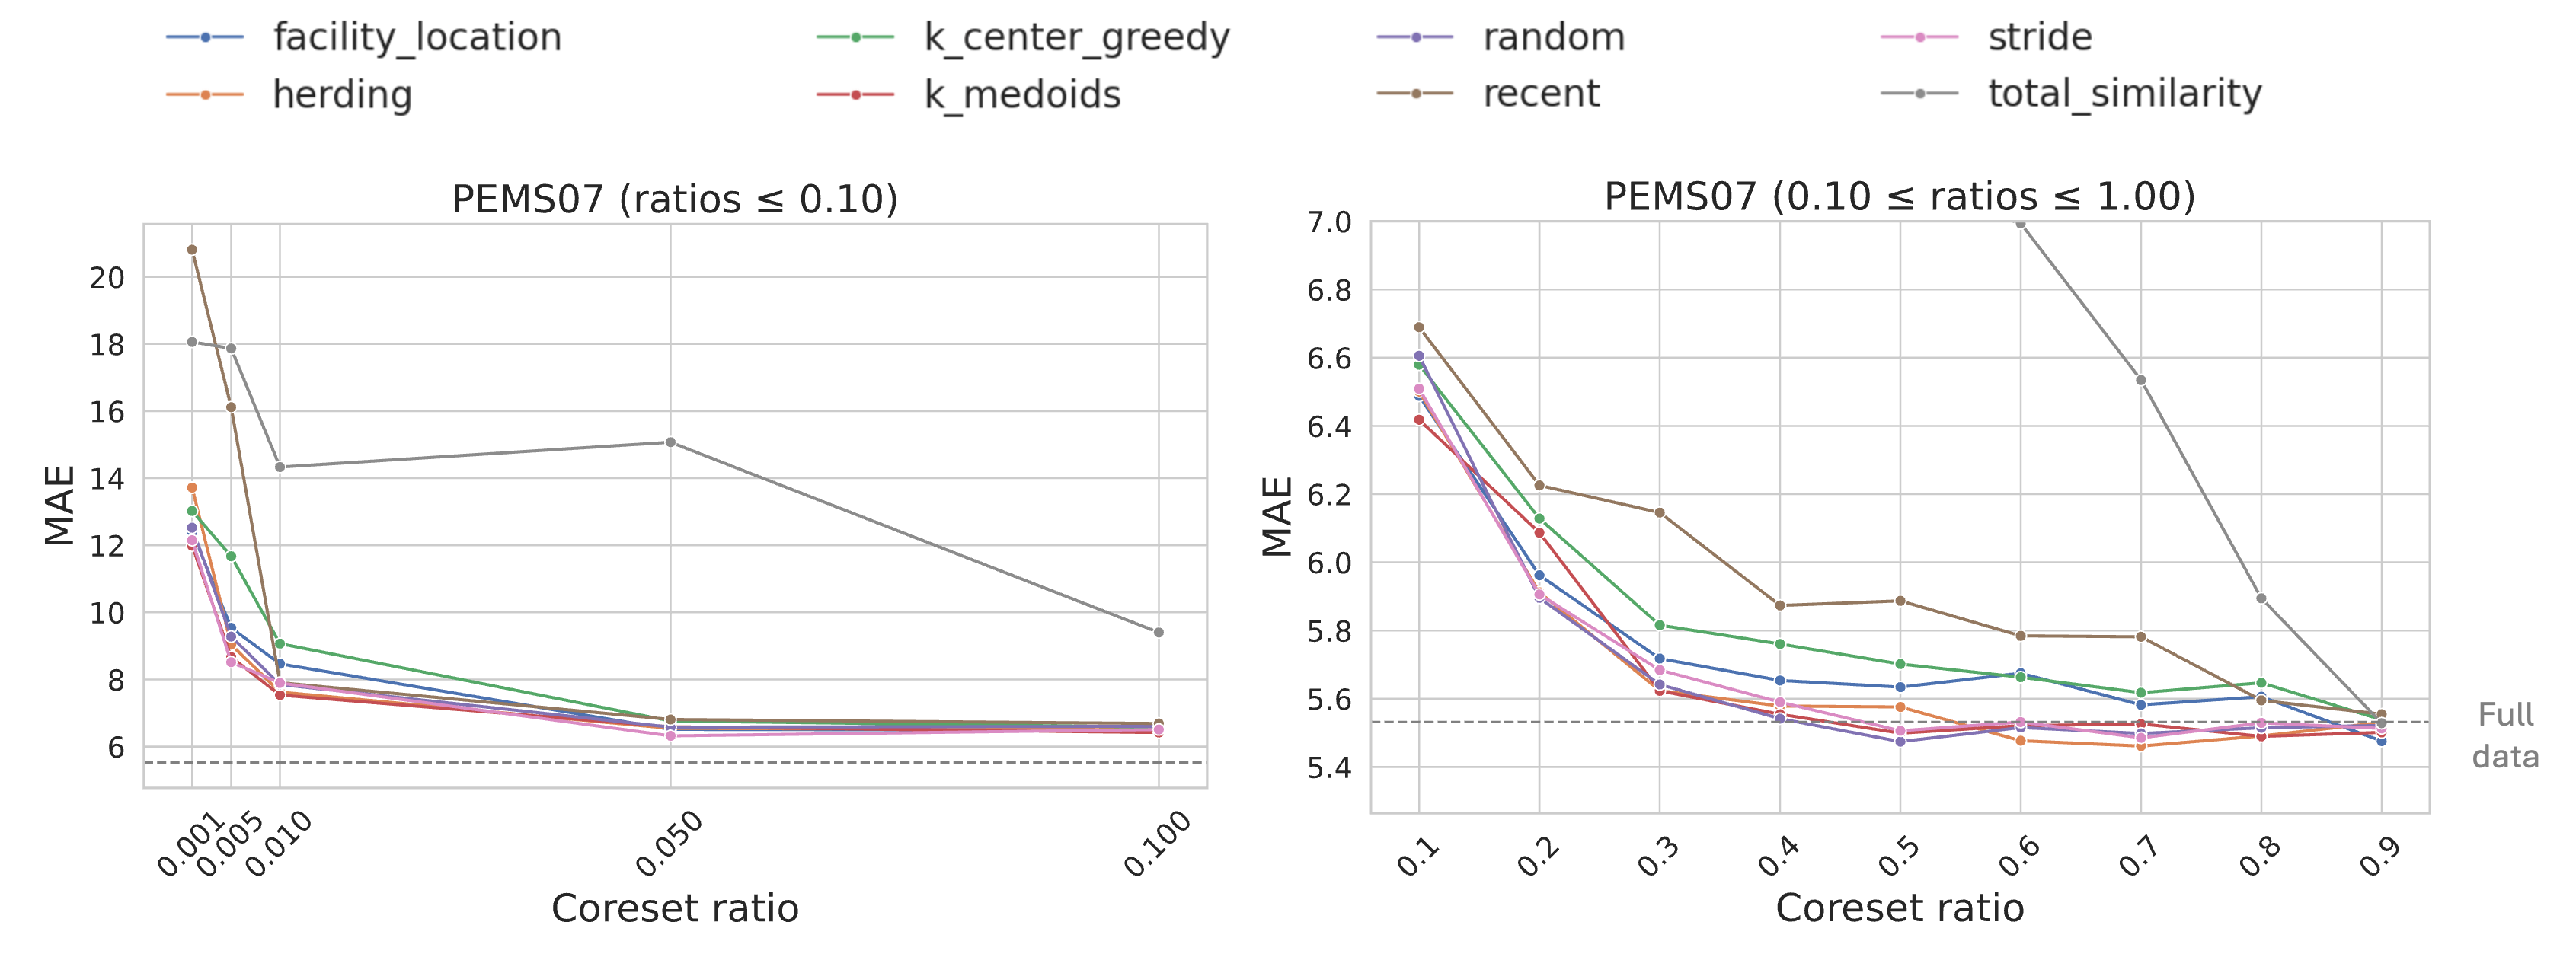
\includegraphics[width=\textwidth]{figures/graph.png} 
  \caption{Overall performance for each selection ratio on PEMS07 dataset} 
  \label{fig:graph}
\end{figure*}

\section{Experiments}

\subsection{Datasets}
We conducted experiments on two traffic datasets collected directly from the Caltrans Performance Measurement System (PeMS)\footnote{\url{https://pems.dot.ca.gov/}}. We selected sensors with consistent latitude/longitude metadata and no null values across three features (speed, occupancy, flow) for selected period.
\begin{itemize}
    \item \textbf{PEMS04-2023}: Contains traffic data collected from Bay Area. This resulted in data from 2,474 sensors across 25,921 5-minute intervals on period from 1 April 2023 to 30 June 2023.
    \item \textbf{PEMS07-2023}: Contains traffic data collected from Los Angeles County. This resulted data from 2,785 sensors across 25,621 5-minute intervals for the period from 1 January 2023 to 31 March 2023.
\end{itemize}


\subsection{Model Architecture}
We utilised the Spatio-Temporal Graph Convolutional Network (STGCN) \cite{yu_spatio-temporal_2018} for all traffic flow forecasting tasks. The input sequence length ($T_{in}$) and the output prediction horizon ($T_{out}$) were set to 12 (representing 60 minutes, given the 5-minute data aggregation).

To model spatial dependencies, we constructed an adjacency matrix $A$ based on  the sensor locations obtained from the metadata. Following the previous work \cite{li_diffusion_2018, liu_largest_2023}, the matrix elements were computed using a thresholded Gaussian kernel:
\begin{equation}
A_{ij} = \begin{cases}
\exp\left(-\frac{\text{dist}(v_i, v_j)^2}{\sigma^2}\right), & \text{if } \exp\left(-\frac{\text{dist}(v_i, v_j)^2}{\sigma^2}\right) \ge 0.1 \\
0, & \text{otherwise}
\end{cases}
\end{equation}
where $\text{dist}(v_i, v_j)$ is the geographical distance between sensors $v_i$ and $v_j$, and $\sigma^2$ was set to the variance of the pairwise distances across all sensors in the respective dataset.

\subsection{Coreset Selection Methods}\label{sec:coreset_methods}
We evaluated eight \textit{model-free} coreset selection approaches. For geometric and submodular methods that require distance or similarity calculations, we used the Euclidean distance calculated directly on the raw input feature vectors ($\mathbf X\!\in\!\mathbb{R}^{N \times T_{\text{in}}\times C}$). No additional embedding or dimensionality reduction techniques were applied to keep the selection process focused on representativeness of raw data.

% \subsection{Coreset Selection Methods}%
% \label{sec:coreset_methods}
% We benchmark eight \emph{training-free} subsetters.  
% Whenever an algorithm requires pairwise affinities we compute plain Euclidean
% distances on the raw tensors
% $\mathbf X\!\in\!\mathbb{R}^{N \times T_{\text{in}}\times C}$; no learnable
% embeddings or dimensionality reduction is introduced, ensuring that g2ains come
% solely from the selection strategy.

\begin{itemize}
    \item \textbf{Random} — uniform sampling.
    \item \textbf{Recent} — the $k$ most recent data points.
    \item \textbf{Stride} — every $m$-th data point along the timeline ($k\!=\!\lfloor\!|D|/m\rfloor$).
    \item \textbf{K-medoids} \cite{kaufmann_clustering_1987} — PAM(Partition Around Medoids) clustering in Euclidean space; the $k$ medoids form the coreset.
    \item \textbf{K-center greedy} \cite{sener_active_2018} — iteratively select the data point that maximises the minimum distance to each step's coreset.
    \item \textbf{Herding} \cite{welling_herding_2009} — sequentially picks data points whose addition best matches the empirical mean of the entire training set.
  \item \textbf{Total Similarity}.  
        For a entire set $\Omega$ and a similarity kernel 
       \[
s_{ij} = \exp\!\left(-\frac{\lVert x_i - x_j \rVert^{2}}{2\sigma^{2}}\right)
\] where $\sigma$ is the median of all pairwise distances,
        the \emph{Total Similarity} function is  
        \[
            f_{\mathrm{TS}}(A)=
            \sum_{i\in\Omega}\sum_{a\in A}s_{ia}
        \]
        iteratively select data point that maximises total similarity objective.

  \item \textbf{Facility-location} \cite{iyer_submodular_2021}.  
        Using the same kernel with Graph-cut, the facility-location function is  
        \[
            f_{\mathrm{FL}}(A)=
            \sum_{i\in\Omega}\max_{a\in A} s_{ia}.
        \]
        iteratively selection data point that maximises facility-location function.
\end{itemize}


\subsection{Experimental Settings}
The data for each dataset were partitioned chronologically into training, validation and test sets as 6:2:2. All experiments were conducted using PyTorch, on AMD MI210, MI300. Input features were normalised using Z-score scaling based on training set statistics.

We evaluated the performance of each coreset selection method by applying the following procedure: For a given coreset selection method and a specified sampling ratio, we first selected a subset of the training data according to the method. The `sampling ratio' represents the proportion of the original training dataset used. For example, a ratio of 0.2 means 20\% of the full training data is selected. Using only the sampled subset, which is the `coreset' identified by the given method, we trained the traffic prediction model from scratch.

Models were trained for a fixed 100 epochs using the Adam optimiser and Mean Absolute Error (MAE) as the loss function. For robustness, all reported results are averaged over 3 independent runs using different random seeds. Performance was measured using Mean Absolute Error (MAE), Root Mean Square Error (RMSE), and Mean Absolute Percentage Error (MAPE), defined as follows:

\begin{equation}
\text{MAE} = \frac{1}{N \times T_{out}} \sum_{i=1}^{N} \sum_{t=1}^{T_{out}} |Y_{i,t} - \hat{Y}_{i,t}|,
\end{equation}

\begin{equation}
\text{RMSE} = \sqrt{\frac{1}{N \times T_{out}} \sum_{i=1}^{N} \sum_{t=1}^{T_{out}} (Y_{i,t} - \hat{Y}_{i,t})^2},
\end{equation}

\begin{equation}
\text{MAPE} = \frac{1}{N \times T_{out}} \sum_{i=1}^{N} \sum_{t=1}^{T_{out}} \left|\frac{Y_{i,t} - \hat{Y}{i,t}}{Y{i,t}}\right| \times 100%,
\end{equation}

where \( Y_{i,t} \) and \( \hat{Y}_{i,t} \) denote the ground truth data and predicted traffic flow for the sensor \( i \) at timestamp \( t \).

% Figure 2: Temporal Distribution Visualization
\begin{figure*}[t]
  \centering
  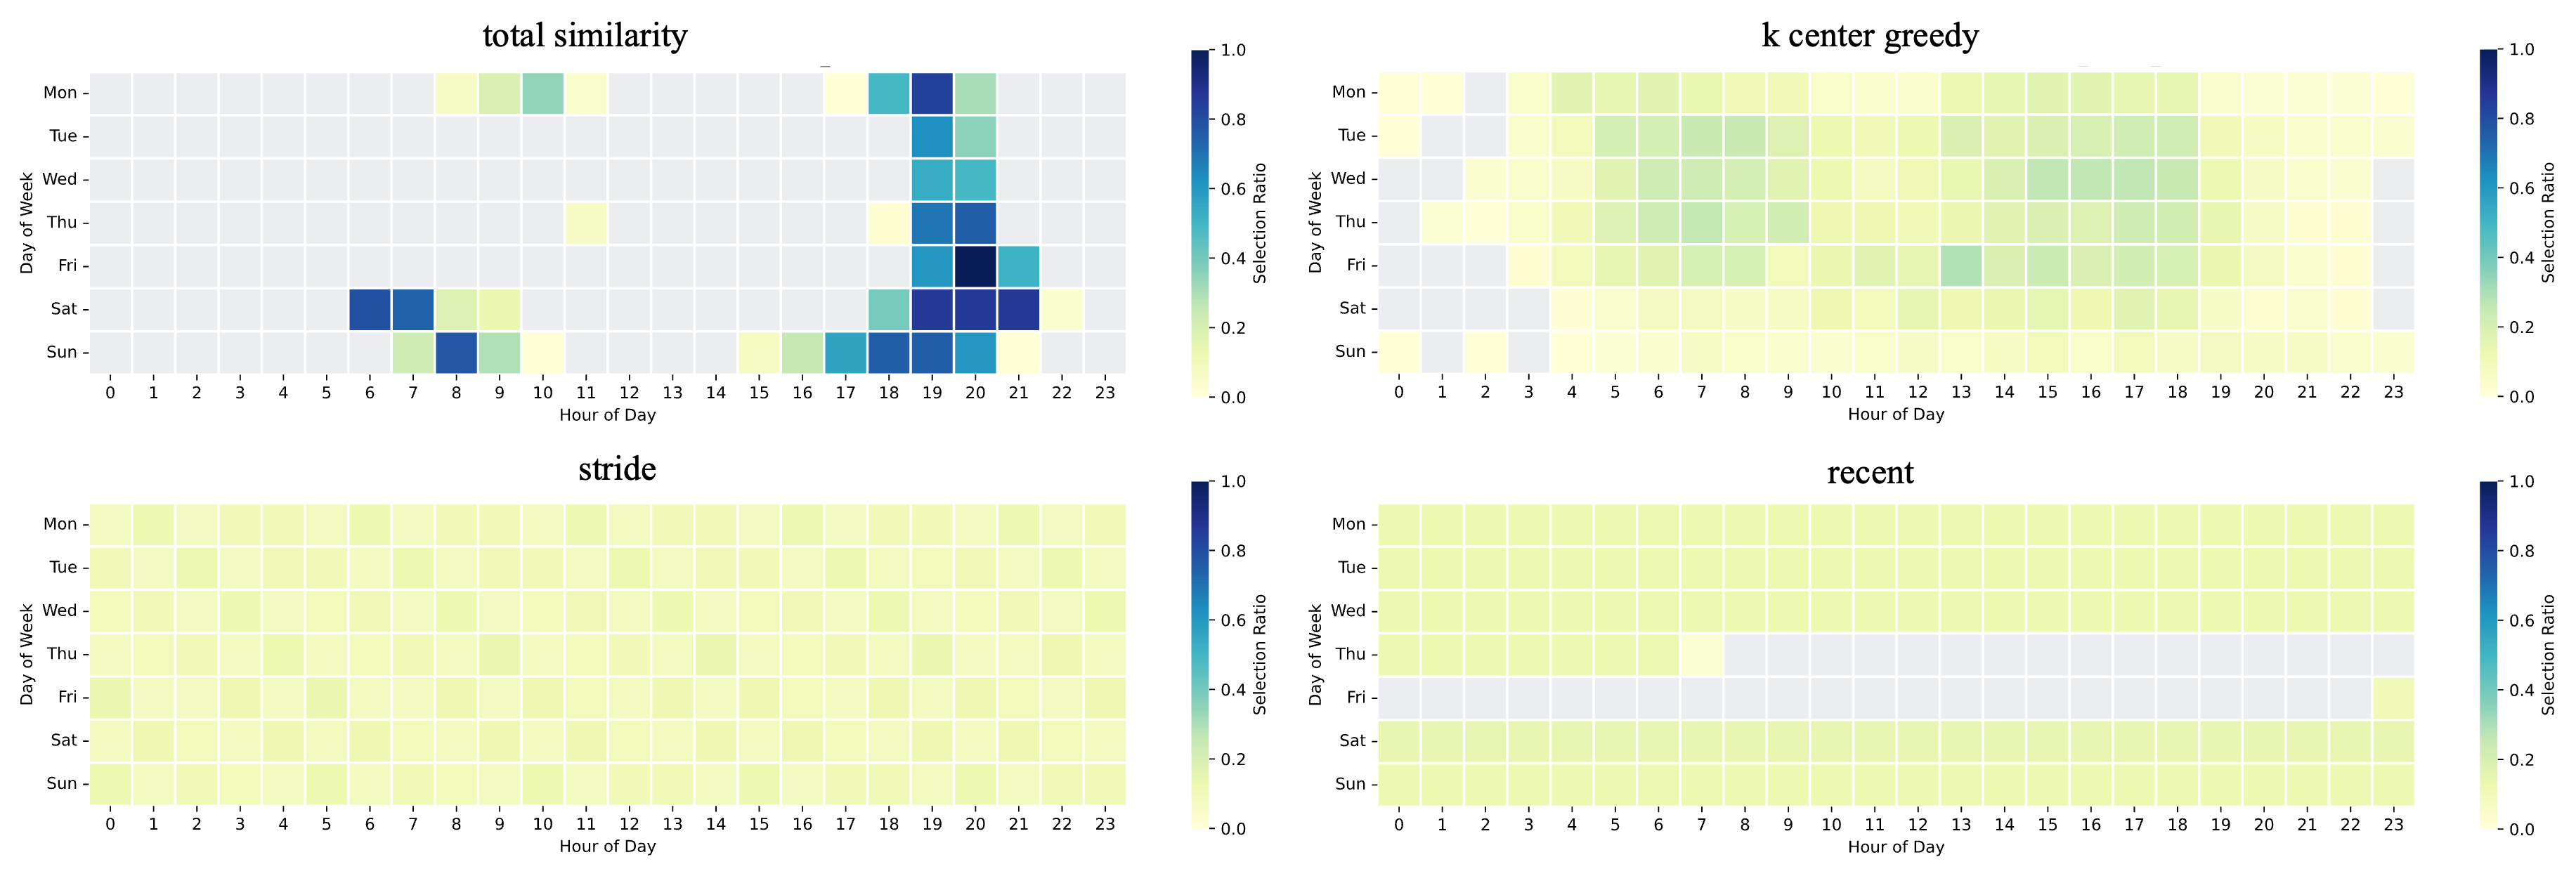
\includegraphics[width=\linewidth]{figures/temporal.png} 
  \caption{Heatmaps showing the temporal distribution (Day of Week vs. Hour of Day) of samples selected by each coreset method, for selection ratio 5\% on PEMS07 dataset. Other methods(Random, Herding, K-medoids, Facility-location) shows even distribution like stride.}
  \label{fig:temporal}
\end{figure*}



\section{Results}

This section presents empirical results from evaluating eight coreset selection methods on the PEMS04 and PEMS07 datasets using the STGCN model.


\subsection{Overall Performance}

Table~\ref{table:full_result} summarises the performance metrics (MAE, RMSE, MAPE) across coreset selection methods and sampling ratios for both PEMS04 and PEMS07 datasets. The results show that coresets enable substantial data reduction while preserving model performance. Performance generally improved (error decreased) as the coreset ratio increased, with several methods achieving near-baseline results using significantly less data. For instance, using only 50\% of the data often achieved errors within 0.1-0.5\% absolute MAPE difference of the full-data baseline, and some methods keep the model performance even at a 30\% ratio. Herding and k-medoids selection for mid-to-high ratio coresets (50-90\%) achieved slightly lower prediction errors than the full-data baseline. Overall, k-medoids selection delivered the most robust and accurate performance across all metrics and datasets.


\begin{table*}[htbp]
\centering
\setlength\tabcolsep{4.3pt}
\renewcommand\arraystretch{1.0}
    \centering
    \caption{Trffic Flow Forecasting on PEMS04 and PEMS07 datasets using coreset selection }
    (\textbf{Bold} denote the best value and \textcolor{blue}{blue} denote the second best in same dataset)
    \label{table:full_result}
    \scalebox{0.83}{
\begin{tabular}{l l l r r r r r r r r r r r r r r r r}
\toprule
 &  & Ratio & Overall rank & Average rank & 0.1\% & 0.5\% & 1\% & 5\% & 10\% & 20\% & 30\% & 40\% & 50\% & 60\% & 70\% & 80\% & 90\% & 100\% \\
\textbf{Data} & \textbf{Method} & \textbf{Metric} &  &  &  &  &  &  &  &  &  &  &  &  &  &  &  &  \\
\midrule
\multirow{24}{*}{\rotatebox{90}{\textbf{PEMS04}}} & \multirow{3}{*}{random} & MAE & \textcolor{blue}{2} & \textcolor{blue}{2.50} & 15.74 & \textcolor{blue}{9.85} & \textcolor{blue}{8.62} & 7.58 & \textcolor{blue}{7.24} & 6.72 & \textbf{6.42} & \textbf{6.32} & \textcolor{blue}{6.28} & 6.26 & 6.25 & 6.28 & \textcolor{blue}{6.21} & \textbf{6.24} \\
 &  & MAPE(\%) & \textcolor{blue}{2} & \textcolor{blue}{2.71} & 69.82 & \textbf{25.87} & \textcolor{blue}{22.80} & 20.50 & 20.37 & \textbf{17.76} & \textbf{16.83} & \textbf{16.68} & 16.80 & \textbf{16.53} & 16.65 & 17.47 & 17.02 & \textbf{16.97} \\
 &  & RMSE & 3 & 2.93 & 35.61 & 23.82 & \textcolor{blue}{21.07} & 18.79 & 17.99 & 17.12 & \textbf{16.59} & \textcolor{blue}{16.42} & \textcolor{blue}{16.34} & 16.35 & 16.32 & 16.30 & \textcolor{blue}{16.22} & \textbf{16.29} \\
\cline{2-19}
 & \multirow{3}{*}{recent} & MAE & 6 & 5.31 & 34.17 & 14.43 & 12.95 & 7.72 & 7.46 & 6.79 & 6.67 & 6.43 & 6.41 & 6.27 & 6.27 & \textbf{6.20} & 6.23 & - \\
 &  & MAPE(\%) & 5 & 4.08 & 75.63 & 34.82 & 34.04 & 20.64 & 20.31 & 18.97 & 18.07 & 17.08 & 17.10 & \textcolor{blue}{16.54} & 16.99 & \textbf{16.44} & \textbf{16.56} & - \\
 &  & RMSE & 6 & 6.08 & 73.07 & 36.30 & 34.51 & 19.08 & 18.56 & 17.29 & 17.13 & 16.70 & 16.63 & 16.36 & 16.37 & 16.27 & 16.32 & - \\
\cline{2-19}
 & \multirow{3}{*}{stride} & MAE & 3 & 2.85 & 16.69 & \textbf{9.50} & 9.10 & \textcolor{blue}{7.54} & \textbf{7.23} & \textbf{6.66} & 6.52 & 6.44 & \textbf{6.27} & \textcolor{blue}{6.24} & 6.31 & 6.26 & \textcolor{blue}{6.21} & - \\
 &  & MAPE(\%) & 4 & 3.31 & 47.98 & 27.29 & 25.14 & 21.13 & \textbf{20.14} & 18.21 & 17.83 & 17.82 & \textbf{16.47} & \textcolor{blue}{16.54} & 17.01 & 16.82 & 16.76 & - \\
 &  & RMSE & \textcolor{blue}{2} & \textcolor{blue}{2.92} & 39.00 & \textbf{23.22} & 21.97 & \textcolor{blue}{18.63} & \textcolor{blue}{17.97} & \textbf{16.97} & 16.71 & 16.54 & \textbf{16.32} & \textcolor{blue}{16.32} & 16.40 & 16.34 & \textbf{16.21} & - \\
\cline{2-19}
 & \multirow{3}{*}{herding} & MAE & 4 & 2.92 & 17.65 & 10.13 & 9.12 & 7.58 & \textcolor{blue}{7.24} & \textbf{6.66} & 6.53 & \textbf{6.32} & 6.34 & \textbf{6.23} & \textcolor{blue}{6.23} & 6.22 & \textbf{6.20} & - \\
 &  & MAPE(\%) & 3 & 3.00 & 48.27 & \textcolor{blue}{26.00} & 23.78 & \textcolor{blue}{20.22} & 20.49 & \textcolor{blue}{17.86} & \textcolor{blue}{17.61} & \textcolor{blue}{16.98} & 16.98 & 16.73 & \textcolor{blue}{16.61} & 16.80 & 16.93 & - \\
 &  & RMSE & 4 & 3.15 & 43.31 & 24.80 & 22.22 & 18.78 & \textbf{17.96} & \textcolor{blue}{17.00} & 16.73 & \textbf{16.40} & 16.45 & \textbf{16.30} & \textcolor{blue}{16.30} & \textcolor{blue}{16.25} & 16.24 & - \\
\cline{2-19}
 & \multirow{3}{*}{k center greedy} & MAE & 7 & 6.46 & \textbf{14.04} & 11.62 & 10.25 & 8.45 & 8.01 & 7.28 & 6.95 & 6.74 & 6.59 & 6.51 & 6.40 & 6.29 & 6.24 & - \\
 &  & MAPE(\%) & 7 & 6.69 & \textcolor{blue}{46.52} & 43.36 & 40.23 & 30.85 & 28.64 & 23.68 & 21.38 & 21.05 & 19.94 & 19.23 & 18.55 & 17.81 & 17.62 & - \\
 &  & RMSE & 6 & 6.08 & \textbf{33.17} & 26.99 & 23.94 & 20.17 & 19.23 & 17.89 & 17.38 & 16.95 & 16.74 & 16.64 & 16.45 & 16.33 & 16.24 & - \\
\cline{2-19}
 & \multirow{3}{*}{k medoids} & MAE & \textbf{1} & \textbf{2.38} & \textcolor{blue}{14.17} & 9.95 & \textbf{8.48} & \textbf{7.44} & 7.29 & 6.72 & \textcolor{blue}{6.47} & 6.42 & 6.29 & 6.27 & \textbf{6.19} & \textbf{6.20} & \textcolor{blue}{6.21} & - \\
 &  & MAPE(\%) & \textbf{1} & \textbf{2.46} & \textbf{43.57} & 29.03 & \textbf{22.08} & \textbf{19.61} & \textcolor{blue}{20.24} & 18.23 & 17.79 & 17.45 & \textcolor{blue}{16.70} & 16.92 & \textbf{16.26} & \textcolor{blue}{16.65} & \textcolor{blue}{16.59} & - \\
 &  & RMSE & \textbf{1} & \textbf{2.62} & \textcolor{blue}{33.82} & 24.17 & \textbf{20.88} & \textbf{18.56} & 18.14 & 17.06 & \textcolor{blue}{16.61} & 16.54 & 16.37 & \textcolor{blue}{16.32} & \textbf{16.22} & \textbf{16.24} & 16.26 & - \\
\cline{2-19}
 & \multirow{3}{*}{facility location} & MAE & 5 & 4.62 & 14.56 & 10.01 & 8.94 & 7.76 & 7.44 & 6.71 & 6.68 & 6.47 & 6.42 & 6.41 & 6.28 & 6.28 & \textcolor{blue}{6.21} & - \\
 &  & MAPE(\%) & 6 & 5.77 & 48.66 & 34.23 & 27.01 & 23.49 & 21.97 & 18.70 & 18.85 & 18.14 & 17.58 & 18.19 & 17.25 & 17.52 & 17.08 & - \\
 &  & RMSE & 5 & 4.00 & 34.36 & \textcolor{blue}{23.54} & 21.68 & 19.00 & 18.38 & 17.06 & 16.97 & 16.60 & 16.56 & 16.48 & \textcolor{blue}{16.30} & 16.31 & 16.23 & - \\
\cline{2-19}
 & \multirow{3}{*}{total similarity} & MAE & 8 & 7.77 & 20.57 & 20.31 & 18.63 & 12.43 & 12.16 & 10.15 & 8.73 & 8.66 & 7.49 & 7.02 & 6.49 & 6.32 & 6.22 & - \\
 &  & MAPE(\%) & 8 & 7.77 & 82.21 & 81.71 & 102.20 & 54.81 & 64.79 & 37.67 & 30.15 & 33.34 & 28.29 & 25.39 & 20.34 & 18.29 & 16.99 & - \\
 &  & RMSE & 8 & 7.54 & 43.13 & 41.97 & 40.14 & 29.14 & 27.77 & 24.79 & 21.51 & 21.21 & 18.89 & 17.66 & 16.68 & 16.38 & 16.24 & - \\
\cline{1-19} \cline{2-19}
\multirow{24}{*}{\rotatebox{90}{\textbf{PEMS07}}} & \multirow{3}{*}{random} & MAE & 3 & 2.86 & 12.53 & 9.28 & 7.85 & 6.58 & 6.61 & \textbf{5.90} & 5.64 & \textbf{5.54} & \textbf{5.47} & \textcolor{blue}{5.52} & 5.50 & 5.51 & 5.52 & \textbf{5.53} \\
 &  & MAPE(\%) & \textcolor{blue}{2} & \textcolor{blue}{2.71} & 35.67 & 23.65 & \textcolor{blue}{19.01} & 15.87 & \textcolor{blue}{16.64} & \textbf{14.40} & 13.46 & 13.13 & \textcolor{blue}{12.59} & 12.89 & 12.59 & 12.53 & \textcolor{blue}{12.46} & \textbf{12.53} \\
 &  & RMSE & 4 & 3.00 & 31.92 & 25.60 & 21.22 & 18.13 & 17.97 & \textcolor{blue}{17.27} & \textcolor{blue}{17.12} & \textcolor{blue}{17.10} & \textbf{17.08} & \textbf{17.27} & \textbf{17.19} & \textbf{17.38} & 17.69 & \textbf{17.75} \\
\cline{2-19}
 & \multirow{3}{*}{recent} & MAE & 7 & 6.85 & 20.81 & 16.12 & 7.91 & 6.81 & 6.69 & 6.23 & 6.15 & 5.87 & 5.89 & 5.78 & 5.78 & 5.60 & 5.55 & - \\
 &  & MAPE(\%) & 6 & 5.54 & 66.81 & 40.81 & 20.47 & 16.17 & 16.83 & 15.43 & 14.37 & 13.92 & 13.97 & 13.53 & 13.24 & 12.86 & 12.73 & - \\
 &  & RMSE & 7 & 6.62 & 50.71 & 41.48 & \textbf{20.13} & 18.72 & 18.50 & 18.59 & 19.26 & 18.40 & 18.74 & 18.40 & 18.68 & 17.79 & 17.75 & - \\
\cline{2-19}
 & \multirow{3}{*}{stride} & MAE & 4 & 2.92 & \textcolor{blue}{12.15} & \textbf{8.52} & 7.90 & \textbf{6.32} & 6.51 & \textcolor{blue}{5.91} & 5.68 & 5.59 & 5.51 & 5.53 & \textcolor{blue}{5.49} & 5.53 & 5.51 & - \\
 &  & MAPE(\%) & \textbf{1} & \textbf{2.23} & \textbf{33.23} & \textbf{20.82} & \textbf{18.94} & \textbf{14.93} & 17.24 & 14.94 & 13.76 & \textcolor{blue}{13.06} & \textbf{12.58} & 12.69 & \textcolor{blue}{12.55} & 12.52 & \textcolor{blue}{12.46} & - \\
 &  & RMSE & \textcolor{blue}{2} & \textcolor{blue}{2.92} & 31.28 & \textcolor{blue}{22.87} & 20.97 & \textbf{17.62} & 17.85 & \textcolor{blue}{17.27} & 17.27 & 17.34 & \textcolor{blue}{17.24} & 17.39 & \textcolor{blue}{17.42} & 17.57 & 17.63 & - \\
\cline{2-19}
 & \multirow{3}{*}{herding} & MAE & \textcolor{blue}{2} & \textcolor{blue}{2.69} & 13.72 & 9.04 & \textcolor{blue}{7.62} & 6.54 & 6.50 & \textcolor{blue}{5.91} & \textbf{5.62} & 5.58 & 5.58 & \textbf{5.48} & \textbf{5.46} & \textbf{5.49} & 5.53 & - \\
 &  & MAPE(\%) & 3 & 2.77 & 37.27 & 22.38 & 19.48 & \textcolor{blue}{15.72} & 16.84 & \textcolor{blue}{14.55} & \textbf{13.09} & \textbf{13.05} & 12.97 & \textbf{12.51} & \textbf{12.31} & \textbf{12.46} & 12.82 & - \\
 &  & RMSE & \textcolor{blue}{2} & \textcolor{blue}{2.92} & 34.03 & 24.49 & 20.66 & 18.00 & 17.93 & \textbf{17.16} & \textbf{17.09} & 17.21 & 17.36 & \textcolor{blue}{17.35} & 17.47 & \textcolor{blue}{17.39} & 17.51 & - \\
\cline{2-19}
 & \multirow{3}{*}{k center greedy} & MAE & 6 & 6.00 & 13.02 & 11.67 & 9.07 & 6.77 & 6.58 & 6.13 & 5.82 & 5.76 & 5.70 & 5.66 & 5.62 & 5.65 & 5.54 & - \\
 &  & MAPE(\%) & 7 & 6.46 & 35.63 & 47.75 & 31.67 & 20.07 & 18.66 & 16.21 & 14.44 & 14.28 & 13.88 & 13.60 & 13.43 & 13.14 & 12.64 & - \\
 &  & RMSE & 6 & 6.00 & 32.07 & 27.86 & 22.82 & 18.29 & 18.01 & 17.76 & 17.56 & 17.80 & 17.83 & 17.76 & 17.82 & 17.97 & 17.65 & - \\
\cline{2-19}
 & \multirow{3}{*}{k medoids} & MAE & \textbf{1} & \textbf{2.23} & \textbf{11.99} & \textcolor{blue}{8.67} & \textbf{7.54} & 6.59 & \textbf{6.42} & 6.09 & \textbf{5.62} & \textcolor{blue}{5.55} & \textcolor{blue}{5.50} & \textcolor{blue}{5.52} & 5.53 & \textbf{5.49} & \textcolor{blue}{5.50} & - \\
 &  & MAPE(\%) & 4 & 3.08 & 35.94 & \textcolor{blue}{21.32} & 19.55 & 16.79 & \textbf{15.12} & 15.35 & \textcolor{blue}{13.45} & 13.26 & 12.77 & \textcolor{blue}{12.62} & 12.67 & \textcolor{blue}{12.49} & \textbf{12.37} & - \\
 &  & RMSE & \textbf{1} & \textbf{2.54} & \textbf{29.90} & \textbf{22.86} & \textcolor{blue}{20.26} & 18.00 & \textcolor{blue}{17.76} & 17.56 & 17.22 & \textbf{17.07} & 17.26 & 17.51 & 17.52 & 17.56 & \textbf{17.40} & - \\
\cline{2-19}
 & \multirow{3}{*}{facility location} & MAE & 5 & 4.23 & 12.41 & 9.54 & 8.47 & \textcolor{blue}{6.51} & \textcolor{blue}{6.49} & 5.96 & 5.72 & 5.65 & 5.63 & 5.67 & 5.58 & 5.61 & \textbf{5.48} & - \\
 &  & MAPE(\%) & 5 & 5.00 & \textcolor{blue}{35.20} & 25.10 & 24.62 & 17.81 & 17.62 & 15.56 & 13.92 & 13.22 & 13.51 & 13.89 & 13.00 & 12.89 & \textcolor{blue}{12.46} & - \\
 &  & RMSE & 5 & 4.00 & \textcolor{blue}{30.92} & 25.16 & 22.01 & \textcolor{blue}{17.77} & \textbf{17.75} & 17.52 & 17.33 & 17.54 & 17.61 & 17.75 & 17.61 & 17.93 & \textcolor{blue}{17.49} & - \\
\cline{2-19}
 & \multirow{3}{*}{total similarity} & MAE & 8 & 7.69 & 18.06 & 17.87 & 14.33 & 15.07 & 9.40 & 8.69 & 7.97 & 7.64 & 7.10 & 6.99 & 6.53 & 5.89 & 5.53 & - \\
 &  & MAPE(\%) & 8 & 7.77 & 64.74 & 42.57 & 52.53 & 52.48 & 26.98 & 27.12 & 22.25 & 24.76 & 21.16 & 22.48 & 20.38 & 15.47 & 12.82 & - \\
 &  & RMSE & 8 & 7.62 & 40.24 & 40.30 & 33.38 & 38.83 & 23.86 & 21.93 & 20.73 & 20.78 & 18.94 & 19.78 & 19.14 & 18.08 & 17.65 & - \\
\cline{1-19} \cline{2-19}

\bottomrule
\end{tabular}
}
\end{table*}


\subsection{Feature Space Coverage and Temporal Distribution}

Figure~\ref{fig:tsne} visualises the coverage of feature space using t-SNE embeddings and KDE, comparing coresets (red) against the full dataset (grey) for the selection ratio 5\%. The quality of this coverage strongly correlates with forecasting accuracy (Table~\ref{table:full_result}). High accuracy methods (Random, Stride, Herding, and K-Medoids) demonstrate representative coverage, while keeping data distribution of entire dataset. In contrast, the poor accuracy of methods (Total Similarity, Recent) corresponds directly to their unbalanced feature space coverage. Consistent with previous coreset selection research in image classification, our findings confirm that better feature space coverage leads to better coreset performance in time-series forecasting problem.



Temporal distribution of coreset samples is also related to the performance of trained model. High accuracy methods(Random, Stride, Herding, K-medoids, Facility Location) generally maintain balanced temporal diversity in terms of day of week and hour of day. It leads to preserve diverse temporal traffic patterns accross different time periods. Conversely, poor accuracy methods (Recent, Total Similarity, K-center-greedy) show unbalanced and biased temporal distribution in the heatmap. Thus, focusing on temporal diversity can be a practical and effective strategy to help achieve the high feature space coverage, offering a simpler alternative to directly handling feature space of complex, high-dimensional data.



\subsection{Discussion}
\subsubsection{Clustering-Based Selection Outperforms at Small Coreset Sampling Ratios
}
In multivariate traffic forecasting under low sampling ratios, a simple geometric distance-based clustering approach achieves strong performance when constructing coresets. This selection constructs a coreset by selecting the center points (medoids) of the data clusters \cite{kaufmann_clustering_1987}. This finding is consistent with previous research \cite{sorscher_beyond_2022}, which shows that retaining 'prototypical' samples rather than 'difficult' ones is more beneficial under low selection ratio. They also showed that a self-supervised prototypicality score, based on k-means centroid distance, outperformed supervised difficulty metrics. These observations suggest that clustering-based algorithms could be useful for measuring sample prototypicality and enable accurate coreset construnction in multivariate time-series domains.




\subsubsection{Coreset Selection Can Increase Model Performance}
Furthermore, we observed several coreset methods that produced slightly lower prediction errors than the entire dataset training baseline. Our observation aligns with previous studies \cite{paul_deep_2021}, \cite{tan_data_2025}, which showed that selective pruning of training samples can increase model accuracy. Our results indicate that coreset selection can perform as data cleaning, potentially removing less informative or confusing samples, on multivariate time-series forecasting.


\subsection{Limitations}
This study has three primary limitations. First, our evaluation involved only the STGCN model and two specific PEMS datasets. Future work will verify these results using datasets of other periods and districts and by applying other models such as Transformer and LSTM to check  whether our findings are broadly applicable.
Second, distances for coreset selection were calculated directly on high-dimensional raw input features.  Meaningful representations of data samples can capture more semantic structure, as suggested by previous work \cite{zheng_coverage-centric_2022}, \cite{xia_moderate_2022}, \cite{maharana_d2_2023}, \cite{tan_data_2025}. Using such representations might enhance the interpretability and effectiveness of coreset selection for high-dimensional traffic datasets.
Third, our current approach prioritizes the selection of representative samples, may lead to reduced representation of rare but meaningful events (e.g., accidents or unusual congestion patterns). By considering overall representativeness, coreset selection may underperform in these uncommon scenarios. Future work could explictly evaluate this risk and explore hybrid approach to capture traffic patterns from unique events.

\subsubsection{Computational Efficiency and Practical Implications}
While this study focuses on data reduction and predictive accuracy, the practical value of coreset selection in real-world ITS deployments hinges on computational efficiency. Coreset selection is lightweight compared to full model training, adding only a one‐time overhead. Once a coreset is constructed, every subsequent training iteration—whether for model updates or hyperparameter tuning—uses a smaller subset, providing continuous savings in compute and memory. This makes coreset reuse especially attractive for iterative development cycles and large‐scale traffic systems.

\section{Conclusion}

We benchmarked eight model-free coreset selection methods on STGCN model for short-term traffic-flow forecasting using the PEMS04 and PEMS07 datasets. Across both datasets, the best methods reduced training data to 30-50\% while keeping MAPE within 0.5 percentage-point of the full-data baseline. In particular, some methods using 70-90\% data sometimes led to better predictive performance than using the full dataset. Our analysis shows that high-performing coresets provide broad feature-space coverage and this can be achieved by preserving temporal diversity. Conversely, coresets containing strong temporal bias performed poorly, providing only limited feature-space coverage by under-sampling certain regions. These insights highlight the value of diversity-aware sampling for computationally data-efficient traffic forecasting. Future work will test the coreset selection on other datasets and different model architectures (e.g., Transformer-based architectures) to confirm how broadly the conclusions hold.




\bibliographystyle{IEEEtran}
\bibliography{references/papers}



\vspace{12pt}

\end{document}

